%%%%%%%%%%%%%%%%%%%%%%%%%%%%%%%%%%%%%%%%%%%%%%%%%%%%%%%%%%%%%%%%%%%%%%
% Lớp 11 | Đạo hàm | Các quy tắc đạo hàm
% Dạng 1D7?2-3: Tiếp tuyến tại một điểm
% Số câu: 75  (sinh tự động bởi tach_cau.py; từ nay thầy sửa trực tiếp file này)
%%%%%%%%%%%%%%%%%%%%%%%%%%%%%%%%%%%%%%%%%%%%%%%%%%%%%%%%%%%%%%%%%%%%%%

%%%%%%%%%%%%%%%% TRẮC NGHIỆM 4 PHƯƠNG ÁN %%%%%%%%%%%%%%%%

% nguồn: Ok_TracNghiemLop11_Lan1
\begin{ex}%[1D7N2-3]%[ma:292198a1]
	Hệ số góc của tiếp tuyến với đồ thị hàm số  $y=\sin x+1$ tại điểm có hoành độ $x_0=\dfrac{\pi}{3}$ là
	\choice 
		 {$k=-\dfrac{\sqrt{3}}{2}$}
		{$k=\dfrac{\sqrt{3}}{2}$} 
		{$k=-\dfrac{1}{2}$} 
		{\True $k=\dfrac{1}{2}$} 
	\loigiai{ 
		Ta có  $y'=\cos x$.\\
		Khi đó hệ số góc của tiếp tuyến với đồ thị hàm số $y=\sin x+1$ tại  điểm có hoành độ $x_0=\dfrac{\pi}{3}$ là $$k=y'\left( \dfrac{\pi}{3} \right)=\cos \dfrac{\pi}{3}=\dfrac{1}{2}.$$
		Vậy  $k=\dfrac{1}{2}$.
	} 
\end{ex}

% nguồn: Ok_TracNghiemLop11_Lan1
\begin{ex}%[1D7N2-3]%[ma:f2d8334e]
	Phương trình  tiếp tuyến với đồ thị hàm số $y=\dfrac{x+2}{x+1}$ tại điểm có hoành độ $x=0$ là?
	\choice 
		 {$y=x+2$}
		{$y=-x-2$} 
		{\True $y=-x+2$} 
		{$y=-x$} 
	\loigiai{Ta có $y(0)=\dfrac{0+2}{0+1}=2$.\\ 
	Ta có $y'=-\dfrac{-1}{(x+1)^2}$. Suy ra  $y'(0)=-\dfrac{1}{(0+1)^2}=-1$.\\
	Phương trình tiếp tuyến với đồ thị hàm số $y=\dfrac{x+2}{x+1}$  tại điểm có hoành độ $x=0$ là
	 $$y=y'(0)(x-0)+y(0)=-1(x-0)+2=-x+2.$$
	} 
\end{ex}

% nguồn: Ok_TracNghiemLop11_Lan1
\begin{ex}%[1D7N2-3]%[ma:7297ef17]
	 Hệ số góc của tiếp tuyến với đồ thị hàm số $f(x)=x^3$ tại điểm $M(-2;-8)$ là?
	 \choice
		{\True  $12$}
		 {$-12$}
		 {$-192$}
		 {$192$}
	\loigiai{Ta có  $f'(x)=3x^2$.\\
	Vậy hệ số góc của tiếp tuyến với đồ thị hàm số $f(x)=x^3$ tại điểm $M(-2;-8)$ là $$f'(-2)=3\cdot (-2)^2=12.$$ 
	} 
\end{ex}

% nguồn: Ok_TracNghiemLop11_Lan1
\begin{ex}%[1D7N2-3]%[ma:ccd8bbc8]
	Cho parabol $(P):y=x^2-3x$. Tiếp tuyến của  $(P)$ đi qua điểm $A(5;10)$ có phương trình là
	\choice 
		 {$y=5x-15$}
		{\True  $y=7x-25$}
		 {$y=x+5$}
		 {$y=3x-5$}
	 \loigiai{
		Ta thấy điểm $A(5;10)$ thuộc parabol  nên $A$ là tiếp điểm.\\
		$y^\prime = 2x-3\Rightarrow  y^\prime (5)=7$.\\
	Phương trình  tiếp tuyến là $y=7x-25$.}
\end{ex}

% nguồn: Ok_Toan11_TracNghiem_Lan2
\begin{ex}%[1D7H2-3]%[ma:9a665fbb]
	Cho hàm số $y=\dfrac{1}{3}x^3+x^2-2x+1$ có đồ thị là $(C)$. Phương trình tiếp tuyến của $(C)$ tại điểm $M\left(1;\dfrac{1}{3}\right)$ là 
	\choice 
		 {$y=3x-2$}
		 {$y=-3x+2$}
		{\True  $y=x-\dfrac{2}{3}$}
		 {$y=-x+\dfrac{2}{3}$}
	\loigiai{ 
		 Ta có $y'=x^2+2x-2$.\\
		 $y'(1)=1$.\\
		Phương trình tiếp tuyến  của $(C)$ tại điểm $M\left(1;\dfrac{1}{3}\right)$ là
		\begin{align*}
			 y=y'(1)(x-1)+\dfrac{1}{3}\Leftrightarrow y=x-1+\dfrac{1}{3}\Leftrightarrow y=x-\dfrac{2}{3}.
		\end{align*}
	 }
\end{ex}

% nguồn: Ok_Toan11_TracNghiem_Lan2
\begin{ex}%[1D7H2-3]%[ma:fe07f6f3]
	Cho hàm số $y=\dfrac{x-2}{x+1}$. Viết phương trình tiếp tuyến của đồ thị hàm số trên tại điểm  có hoành độ $x_0=0$.
	\choice 
		{\True $y=3x-2$} 
		 {$y=-3x-2$}
		 {$y=3x-3$}
		{$y=3x+2$} 
	 \loigiai{
		 Tập xác định $\mathscr{D}=\mathbb{R}\setminus\left\{-1\right\}$.\\
		$y=\dfrac{x-2}{x+1}\Rightarrow y'=\dfrac{3}{(x+1)^2}$.\\ 
		$y(0)=-2$, $y'(0)=3$.\\ 
		Suy ra phương  trình tiếp tuyến của đồ thị hàm số trên tại điểm có hoành độ $x_0=0$ là
		\begin{align*}
			y=3(x-0)-2\Leftrightarrow  y=3x-2.
		\end{align*}
	} 
\end{ex}

% nguồn: Ok_Toan11_TracNghiem_Lan2
\begin{ex}%[1D7H2-3]%[ma:88d65738]
	Viết phương trình tiếp tuyến của đồ  thị $(C)\colon y=x^4-8x^2+9$ tại điểm $M$ có hoành độ bằng $-1$.
	 \choice
		{\True  $y=12x+14$}
		{$y=12x-14$} 
		{$y=12x+10$} 
		{$y=-20x-22$} 
	 \loigiai{
		Tập  xác định $\mathbb{R}$.\\
		$y'=4x^3-16x$. Suy ra  $y'(-1)=12$.\\
		Ta  có $y(-1)=2$.\\
		Tiếp  tuyến của đồ thị $(C)$ tại $M(-1;2)$ có phương trình là
		\begin{align*}
			 y=12(x+1)+2\Leftrightarrow y=12x+14.
		\end{align*}
	} 
\end{ex}

% nguồn: Ok_Toan11_TracNghiem_Lan2
\begin{ex}%[1D7H2-3]%[ma:68f449d4]
	Cho hàm số $y=\dfrac{x+1}{x-1}$ có đồ thị $(C)$.  Gọi $d$ là tiếp tuyến của $(C)$ tại điểm có tung độ bằng $3$. Tìm hệ số góc $k$ của đường thẳng $d$.
	\choice 
		{$-\dfrac{1}{2}$} 
		{\True $-2$} 
		 {$2$}
		 {$\dfrac{1}{2}$}
	\loigiai{ 
		\begin{itemize}
			\item Với $y=3$, ta có $\dfrac{x+1}{x-1}=3$. Suy ra $x=2$. 
			\item  Ta có $y'=-\dfrac{2}{(x-1)^{2}}$.
			\item Hệ số góc của tiếp tuyến tại điểm có hoành độ bằng $2$ là  $k=y'(2)=-\dfrac{2}{(2-1)^{2}}=-2$.
		\end{itemize}
	} 
\end{ex}

% nguồn: Ok_Toan11_TracNghiem_Lan2
\begin{ex}%[1D7H2-3]%[ma:bfe02dc9]
	Phương trình tiếp tuyến của đồ thị hàm số $y=\dfrac{-x+3}{x-1}$  tại điểm có hoành độ $x=0$ là
	 \choice
		{$y=-2x+3$} 
		{\True  $y=-2x-3$}
		 {$y=2x-3$}
		{$y=2x+3$} 
	 \loigiai{
		Tập  xác định $\mathscr{D}=\mathbb{R}\setminus\left\{1\right\}$.\\
		 $y'=\dfrac{-2}{(x-1)^2}\Rightarrow y'(0)=-2$.\\
		Với  $x=0\Rightarrow y=-3$.\\
		Phương trình  tiếp tuyến cần tìm là $y=-2x-3$.
	} 
\end{ex}

% nguồn: Ok_Toan11_TracNghiem_Lan2
\begin{ex}%[1D7H2-3]%[ma:5084384d]
	Tiếp tuyến của đồ thị hàm số $y=\dfrac{x+1}{x-1}$ tại điểm $A(2;3)$ có phương  trình $y=ax+b$. Tính $a+b$.
	 \choice
		 {$9$}
		 {\True $5$}
		 {$1$}
		 {$-1$}
	 \loigiai{
		Điều kiện  $x\neq 1$.\\
		Ta có  $y'=\dfrac{-2}{(x-1)^2}\Rightarrow y'(2)=-2$.\\
		Phương trình tiếp tuyến  tại điểm $A(2;3)$ là $y=-2(x-2)+3=-2x+7$.\\
		Do đó,  $a=-2$, $b=7$.\\
		Vậy $a+b=5$. 
	} 
\end{ex}

% nguồn: Ok_Toan11_TracNghiem_Lan2
\begin{ex}%[1D7H2-3]%[ma:504dd5b0]
	Tiếp tuyến của đồ thị hàm số $y=\dfrac{-x+1}{3x-2}$ tại giao điểm của đồ thị hàm số với  trục tung có hệ số góc là
	 \choice
		{$-1$} 
		 {$\dfrac{1}{4}$}
		{$\dfrac{5}{4}$} 
		 {\True $-\dfrac{1}{4}$}
	\loigiai{ 
		Ta  có $y'=\dfrac{-1}{(3x-2)^2}$.\\
		Gọi $M$ là tọa độ giao điểm của đồ thị hàm số với trục tung.  Khi đó, $M\left(0;-\dfrac{1}{2}\right)$.\\
		 Vậy hệ số góc cần tìm là $k=y'(0)=-\dfrac{1}{4}$.
	 }
\end{ex}

% nguồn: Ok_Toan11_TracNghiem_Lan2
\begin{ex}%[1D7H2-3]%[ma:b5a8f33e]
	Cho hàm số $y=x^4+2x^2+1$ có đồ thị $(C)$. Phương trình tiếp tuyến của đồ thị $(C)$ tại điểm $M(1;4)$ là 
	 \choice
		 {\True $y=8x-4$}
		 {$y=x+3$}
		{$y=-8x+12$} 
		{$y=8x+4$} 
	\loigiai{ 
		Ta  có $y'=4x^3+4x\Rightarrow y'(1)=8$.\\
		Vậy phương trình tiếp tuyến cần  tìm là $y=8(x-1)+4=8x-4$.
	} 
\end{ex}

% nguồn: Ok_Toan11_TracNghiem_Lan2
\begin{ex}%[1D7H2-3]%[ma:eec65d6d]
	Tiếp tuyến của đồ thị hàm số $y=\dfrac{x+1}{2x-3}$ tại điểm có hoành độ $x_0=-1$ có hệ  số góc bằng
	 \choice
		 {$5$}
		 {\True $-\dfrac{1}{5}$}
		{$-5$} 
		 {$\dfrac{1}{5}$}
	\loigiai{ 
		Tập xác  định của hàm số $y=\dfrac{x+1}{2x-3}$ là $\mathscr{D}=\mathbb{R}\setminus\left\{\dfrac{3}{2}\right\}$.\\
		 Ta có $f'(x)=\dfrac{-5}{(2x-3)^2}$.\\
		Hệ số  góc của tiếp tuyến của đồ thị hàm số tại điểm có hoành độ $x_0=-1$ là
		\begin{align*}
			f'(-1)=\dfrac{-5}{\left[2\cdot (-1)-3\right]^2}=\dfrac{-5}{(-5)^2}=-\dfrac{1}{5}. 
		\end{align*}
	} 
\end{ex}

% nguồn: Ok_Toan11_TracNghiem_Lan2
\begin{ex}%[1D7H2-3]%[ma:53bebf15]
	Hệ số góc tiếp tuyến tại $A(1;0)$ của đồ  thị hàm số $y=x^3-3x^2+2$ là
	\choice 
		 {$1$}
		 {$-1$}
		 {\True $-3$}
		 {$0$}
	\loigiai{ 
		 $y=f(x)=x^3-3x^2+2\Rightarrow f '(x)=3x^2-6x$.\\
		Hệ số góc tiếp  tuyến tại $A(1;0)$ của đồ thị hàm số $y=x^3-3x^2+2$ là $f '(1)=3\cdot 1^2-6\cdot 1=-3$.
	} 
\end{ex}

% nguồn: Ok_Toan11_TracNghiem_Lan2
\begin{ex}%[1D7H2-3]%[ma:43c2450f]
	Viết phương trình  tiếp tuyến của đồ thị hàm số $y=x^4-4x^2+5$ tại điểm có hoành độ $x_0=-1$.
	 \choice
		{$y=4x-6$} 
		{$y=4x+2$} 
		 {\True $y=4x+6$}
		 {$y=4x-2$}
	 \loigiai{
		Ta có $y'=4x^3-8x$. Suy ra  $y'(-1)=4$.\\
		Điểm thuộc đồ  thị đã cho có hoành độ $x_0=-1$ là $M(-1;2)$.\\
		Vậy phương trình tiếp tuyến của đồ thị hàm  số tại $M(-1;2)$ là
		\begin{align*}
			y=y'(-1)(x+1)+2\Leftrightarrow y=4(x+1)+2\Leftrightarrow y=4x+6. 
		\end{align*}
	} 
\end{ex}

% nguồn: Ok_Toan11_TracNghiem_Lan2
\begin{ex}%[1D7H2-3]%[ma:12aec167]
	Cho hàm số $y=-x^3+3x-2$ có đồ thị $(C)$. Viết phương trình tiếp tuyến của $(C)$ tại giao điểm của $(C)$ với trục tung. 
	 \choice
		{$y=-2x+1$} 
		 {$y=2x+1$}
		 {\True $y=3x-2$}
		 {$y=-3x-2$}
	 \loigiai{
		Ta  có $y'=-3x^2+3$.\\
		Giao điểm của $(C)$  với trục tung có tọa độ là $(0;-2)$.\\
		Ta có  $y'(0)=3$.\\
		Tiếp tuyến của $(C)$ tại điểm $(0;-2)$  có phương trình là
		\begin{align*}
			 y=3(x-0)-2\Leftrightarrow y=3x-2.
		\end{align*}
	} 
\end{ex}

% nguồn: Ok_Toan11_TracNghiem_Lan2
\begin{ex}%[1D7H2-3]%[ma:285f9de9]
	Phương trình  tiếp tuyến của đồ thị hàm số $y=\dfrac{3x-1}{x-1}$ tại điểm có hoành độ $x=2$ là
	 \choice
		{$y=2x+9$} 
		{\True  $y=-2x+9$}
		 {$y=2x-9$}
		 {$y=-2x-9$}
	\loigiai{ 
		Ta có $y'=\dfrac{-2}{(x-1)^2}$,  $y'(2)=-2$.\\
		Khi  $x=2$ thì $y=5$.\\
		Phương trình  tiếp tuyến của đồ thị hàm số $y=\dfrac{3x-1}{x-1}$ tại điểm có hoành độ $x=2$ là
		\begin{align*}
			y=-2(x-2)+5\Leftrightarrow  y=-2x+9.
		\end{align*}
	} 
\end{ex}

% nguồn: Ok_Toan11_TracNghiem_Lan2
\begin{ex}%[1D7H2-3]%[ma:9a83423b]
	 Viết phương trình tiếp tuyến của đồ thị hàm số $y=x^4-6x^2+5$ tại điểm có hoành độ $x=2$.
	\choice 
		 {$y=-8x-16$}
		{\True $y=8x-19$} 
		 {$y=-8x+16$}
		{$y=8x+19$} 
	\loigiai{ 
		Ta có $y(2)=2^4-6\cdot  2^2+5=-3$.\\
		$y'=4x^3-12x\Rightarrow  y'(2)=4\cdot (2)^3-12\cdot 2=8$.\\
		Phương trình tiếp tuyến của đồ thị hàm số là 
		\begin{align*}
			 y=y'(2)\cdot (x-2)+y(2)\Leftrightarrow y=8(x-2)-3\Leftrightarrow y=8x-19.
		\end{align*}
	} 
\end{ex}

% nguồn: Ok_Toan11_TracNghiem_Lan2
\begin{ex}%[1D7H2-3]%[ma:72dfee14]
	Phương trình tiếp tuyến của đồ thị $(H)\colon y=\dfrac{x-1}{x+2}$ tại giao điểm của $(H)$ và  trục hoành là
	 \choice
		 {$y=x-3$}
		{\True $y=\dfrac{1}{3}(x-1)$} 
		 {$y=3x$}
		 {$y=3(x-1)$}
	 \loigiai{
		Giao điểm của $(H)$  và trục hoành là điểm $M(1;0)$.\\
		 Ta có $y'=\dfrac{3}{(x+2)^2}$ nên $y'(1)=\dfrac{1}{3}$.\\
		Phương trình tiếp tuyến với  $(H)$ tại điểm $M$ là
		\begin{align*}
			y=\dfrac{1}{3}(x-1)+0\Leftrightarrow  y=\dfrac{1}{3}(x-1).
		\end{align*}
	} 
\end{ex}

% nguồn: Ok_Toan11_TracNghiem_Lan2
\begin{ex}%[1D7H2-3]%[ma:e738bd5b]
	Gọi $I$ là giao điểm giữa đồ thị hàm số $y=\dfrac{x+1}{x-1}$ và trục tung của hệ trục tọa độ $Oxy$. Hệ số góc của tiếp tuyến với  đồ thị hàm số trên tại $I$ là
	 \choice
		{\True  $-2$}
		 {$0$}
		 {$-1$}
		 {$2$}
	 \loigiai{
		Tập xác định  $\mathscr{D}=\mathbb{R}\setminus\left\{1\right\}$.\\
		Ta có  $y'=\dfrac{-2}{(x-1)^2}$.\\
		Theo  bài ra ta có $I(0;-1)$.\\
		Hệ số góc của tiếp tuyến với đồ  thị hàm số tại $I$ là $y'(0)=\dfrac{-2}{(0-1)^2}=-2$.
	} 
\end{ex}

% nguồn: Ok_Toan11_TracNghiem_Lan2
\begin{ex}%[1D7H2-3]%[ma:cbf8ca3c]
	Viết phương trình tiếp tuyến của đồ thị hàm số $y=x^3-3x$ tại điểm có hoành  độ bằng $2$.
	 \choice
		 {$y=-9x+16$}
		 {$y=-9x+20$}
		{$y=9x-20$} 
		 {\True $y=9x-16$}
	\loigiai{ 
		Tập  xác định $\mathscr{D}=\mathbb{R}$.\\
		 Đạo hàm $y'=3x^2-3$.\\
		 Ta có $y(2)=2$ và $y'(2)=9$.\\
		Do đó, phương trình tiếp tuyến cần tìm  là
		\begin{align*}
			y=9(x-2)+2\Leftrightarrow  y=9x-16.
		\end{align*}
	} 
\end{ex}

% nguồn: Ok_Toan11_TracNghiem_Lan2
\begin{ex}%[1D7H2-3]%[ma:91de5d0d]
	Cho hàm số $y=x^3-2x+1$ có đồ thị $(C)$. Hệ số góc $k$ của tiếp tuyến với $(C)$ tại điểm  có hoành độ $x_0=1$ là
	 \choice
		 {$k=-5$}
		{$k=10$} 
		{$k=25$} 
		 {\True $k=1$}
	 \loigiai{
		Ta  có $y'=3x^2-2$.\\
		Hệ số góc $k$ của tiếp tuyến với  $(C)$ tại điểm có hoành độ $x_0=1$ là $k=y'(1)=1$.
	 }
\end{ex}

% nguồn: Ok_Toan11_TracNghiem_Lan2
\begin{ex}%[1D7H2-3]%[ma:13ad324a]
	Cho hàm số $y=\dfrac{x-m}{x+1}$ có đồ thị là $(C_m)$. Với giá trị nào của $m$ thì tiếp tuyến của $(C_m)$ tại điểm có hoành độ bằng $0$  song song với đường thẳng $d\colon y=3x+1$?
	\choice 
		 {$m=3$}
		 {\True $m=2$}
		{$m=1$} 
		{$m=-2$} 
	 \loigiai{
		Tập xác định: $\mathscr{D}=\mathbb{R}\setminus\left\{-1\right\}$.\\ 
		Ta có $y'=\dfrac{m+1}{(x+1)^2}$.\\ 
		Gọi $M(0;-m)\in(C_m)$; $k$ là  hệ số góc của tiếp tuyến của $(C_m)$ tại $M$ và $d\colon y=3x+1$.\\
		Do tiếp tuyến tại $M$ song song với  $d$ nên
		\begin{align*}
			 k=3\Leftrightarrow y'(0)=3\Leftrightarrow m+1=3\Leftrightarrow m=2.
		\end{align*}
		Khi $m=2$, ta được $M(0;-2)$. Phương  trình tiếp tuyến của đồ thị tại $M(0;-2)$ là
		\begin{align*}
			 y=3(x-0)+(-2)\Leftrightarrow y=3x-2.
		\end{align*}
		Vậy $m=2$ thỏa mãn yêu cầu bài toán. 
	 }
\end{ex}

% nguồn: Ok_Toan11_TracNghiem_Lan2
\begin{ex}%[1D7H2-3]%[ma:c67d0bce]
	Phương trình tiếp tuyến của đồ thị $(C)\colon y=3x-4x^2$ tại điểm có hoành độ  $x_0=0$ là
	\choice 
		 {$y=0$}
		{\True $y=3x$} 
		 {$y=3x-2$}
		 {$y=-12x$}
	 \loigiai{
		Tập  xác định $\mathscr{D}=\mathbb{R}$.\\
		 Đạo hàm $y'=3-8x$.\\
		Ta có  $y(0)=0$ và $y'(0)=3$.\\
		 Phương trình tiếp tuyến là
		\begin{align*}
			y=3(x-0)+0\Leftrightarrow  y=3x.
		\end{align*}
	 }
\end{ex}

% nguồn: Ok_Toan11_TracNghiem_Lan2
\begin{ex}%[1D7H2-3]%[ma:93ad63d7]
	Viết phương trình tiếp tuyến của đồ thị  $y=x^2+x-2$ tại điểm có hoành độ $x_0=-1$.
	 \choice
		{$x+y-1=0$} 
		{$x-y-2=0$} 
		{\True $x+y+3=0$} 
		 {$x-y-1=0$}
	\loigiai{ 
		 Đặt $y=f(x)=x^2+x-2$.\\
		 Ta có $y'=f'(x)=2x+1$.\\
		Tại $x_0=-1\Rightarrow\heva{& f'(-1)=-1\\ &y_0=f(-1)=-2.}$\\ 
		Vậy phương trình tiếp  tuyến cần tìm là
		\begin{align*}
			y=-1(x+1)-2\Leftrightarrow x+y+3=0. 
		\end{align*}
	 }
\end{ex}

% nguồn: Ok_Toan11_TracNghiem_Lan2
\begin{ex}%[1D7H2-3]%[ma:99e70d13]
	Tiếp tuyến của đồ thị hàm số $y=\dfrac{2x+3}{x-2}$  tại điểm có hoành độ bằng $3$, tương ứng là
	 \choice
		 {$y=7x+13$}
		{\True $y=-7x+30$} 
		 {$y=3x+9$}
		{$y=-x-2$} 
	\loigiai{ 
		Ta  có $x=3\Rightarrow y=9$.\\
		 $y'=\dfrac{-7}{(x-2)^2}\Rightarrow y'(3)=-7$.\\
		Phương trình tiếp tuyến tương  ứng là
		\begin{align*}
			y=-7(x-3)+9\Leftrightarrow y=-7x+30. 
		\end{align*}
	 }
\end{ex}

% nguồn: Ok_TracNghiemLop11_Lan1
\begin{ex}%[1D7H2-3]%[5-CTST]%[ma:b02d75cd]
	Đạo hàm của hàm số $y = 5\sin{x} -  3\cos{x}$ tại $x_0 = \dfrac{\pi}{2}$ là
	\choice 
		{\True $y'\left(\dfrac{\pi}{2}  \right) = 3$}
		 {$y'\left(\dfrac{\pi}{2} \right) = 5$}
		{$y'\left(\dfrac{\pi}{2} \right) =  -3$}
		{$y'\left(\dfrac{\pi}{2}  \right) = -5$}
	 \loigiai{
		Ta có $y' =  5\cos{x} + 3\sin{x} \Rightarrow y\left(\dfrac{\pi}{2} \right) = 3$.
	 }
\end{ex}

% nguồn: Ok_TracNghiemLop11_Lan1
\begin{ex}%[1D7H2-3]%[ma:d809fbf8]
	 Cho hàm số $y=x^3-x-1$ có đồ thị $(C)$. Phương trình tiếp tuyến của $(C)$ tại giao điểm của $(C)$ với trục tung là
	\choice 
		{$y=-x-1$} 
		{\True  $y=-x+1$}
		 {$y=2x+2$}
		 {$y=2x-1$}
	\loigiai{ 
		Gọi tiếp điểm $M(x_0;y_0)$. Vì $M(x_0;y_0)$ là giao  điểm của $(C)$ với trục tung nên $M(0;-1)$.\\
		Hệ số  góc của tiếp tuyến là $y'(0)=3\cdot 0^2-1=-1$.\\
	Vậy phương trình tiếp tuyến là $y=y'(0)\left( x-x_0\right)+y_0\Leftrightarrow  y=-x+1$.}
\end{ex}

% nguồn: Ok_TracNghiemLop11_Lan1
\begin{ex}%[1D7H2-3]%[ma:add141c1]
	Viết phương trình tiếp tuyến của đồ thị  hàm số $f(x)=x^3-2x^2+3x+1$ tại điểm có hoành độ $x_0=2$.
	 \choice
		 {$y=-x-7$}
		{$y=7x-14$} 
		 {\True $y=7x-7$}
		 {$y=-x+9$}
	\loigiai{ 
		Với $x_0=2$ ta  có $y_0=f(x_0)=7$. \\
		 Và $f'(x)=3x^2-4x+3 \Rightarrow f'(2)=7$. \\
	 Vậy phương trình tiếp tuyến cần tìm là $y=f'(2)(x-2)+7\Leftrightarrow y=7x-7$.}
\end{ex}

% nguồn: Ok_TracNghiemLop11_Lan1
\begin{ex}%[1D7H2-3]%[ma:fb140803]
	Viết phương trình tiếp tuyến của đồ thị hàm số  $y=x^3-3x$ tại điểm có hoành độ bằng $2$.
	\choice 
		 {$y=-9x+16$}
		 {$y=-9x+20$}
		 {$y=9x-20$}
		 {\True$y=9x-16$}
	 \loigiai{
		\begin{itemize}
			\item  $y'=3x^2-3$.
			\item Ta có $y\left(2\right)=2$ và  $y'\left(2\right)=9$.
			 \item Phương trình tiếp tuyến tại điểm $M(2; 2)$ là $y=9\left(x-2\right)+2\Leftrightarrow y=9x-16$.
		\end{itemize}
	} 
\end{ex}

% nguồn: Ok_TracNghiemLop11_Lan1
\begin{ex}%[1D7H2-3]%[ma:b80af468]
	Phương trình tiếp tuyến của đồ thị $(C)\colon y=3x-4x^2$ tại  điểm có hoành độ $x_{0}=0$ là
	 \choice
		{$y=0$} 
		 {\True $y=3x$}
		{$y=3x-2$} 
		 {$y=-12x$}
	 \loigiai{
		Tập xác định $D=\mathbb{R}$.\\ 
		Ta có $y(0)=0$. Đạo hàm $y'=3-8x$; $y'(0)=3$.\\ 
		Phương trình tiếp tuyến của $(C)$ tại $(0;0)$ là $y=y'_{(0)}\cdot(x-0)+y_{(0)}=3(x-0)+0=3x$. 
	} 
\end{ex}

% nguồn: Ok_Toan11_TracNghiem_Lan2
\begin{ex}%[1D7V2-3]%[ma:4af66a56]
	Cho hàm số $y=-x^3+3x^2+9x-1$ có đồ thị $(C)$. Hệ số góc lớn nhất của tiếp tuyến với đồ  thị là
	 \choice
		 {$1$}
		{$6$} 
		{\True  $12$}
		 {$9$}
	\loigiai{ 
		 Hàm số $y=-x^3+3x^2+9x-1$ có tập xác định $\mathscr{D}=\mathbb{R}$.\\
		Ta có $y'=-3x^2+6x+9=12-3(x-1)^2\leq 12$.\\ 
		Dấu \lq\lq$=$\rq\rq~xảy ra khi và  chỉ khi $x=1$.\\
		Vậy hệ  số góc lớn nhất của tiếp tuyến với đồ thị hàm số là $12$.
	} 
\end{ex}

% nguồn: Ok_Toan11_TracNghiem_Lan2
\begin{ex}%[1D7V2-3]%[ma:b0d3b77c]
	Cho hàm số $y=\dfrac{1}{x-1}$ có đồ thị $(C)$. Gọi $\Delta$ là tiếp tuyến của $(C)$ tại điểm $M(2;1)$. Diện tích tam giác được tạo bởi  $\Delta$ và các trục tọa độ bằng
	 \choice
		{$3$} 
		{$\dfrac{3}{2}$} 
		{$9$} 
		 {\True $\dfrac{9}{2}$}
	 \loigiai{
		\begin{itemize}
			 \item $y'=\dfrac{-1}{(x-1)^{2}}$.
			\item Tại $x_{0}=2$. Suy ra  $y'(2)=-1$.
			\item Phương trình tiếp tuyến $\Delta$  là $y=-(x-2)+1 \Leftrightarrow y=-x+3$.
			\item Tiếp tuyến $\Delta$ cắt các trục $Ox$, $Oy$ lần  lượt tại $A(3;0)$, $B(0;3)$.
			\item Diện tích tam giác $OAB$ là $S=\dfrac{1}{2} \cdot OA \cdot OB = \dfrac{1}{2} \cdot 3 \cdot 3  = \dfrac{9}{2}$.
		\end{itemize}
	} 
\end{ex}


%%%%%%%%%%%%%%%% ĐÚNG/SAI %%%%%%%%%%%%%%%%

% nguồn: Ok_dungsai_lop11_Lan1
\begin{ex}%[1D7N2-3]%[ma:61bc350d]
  Cho hàm số $y=\dfrac{x}{x+1}$ có đồ thị $(C)$. Hãy xét tính đúng, sai của các mệnh đề sau
 \choiceTF 
  {\True Hệ số góc của tiếp tuyến của đồ thị $(C)$  tại điểm $M(-2;2)$ là $1$}
  {Hệ số góc của tiếp tuyến của  đồ thị $(C)$ tại điểm có hoành độ $x=1$ là $\dfrac{1}{2}$}
  {\True  Phương trình tiếp tuyến của đồ thị $(C)$ tại điểm $A(0,0)$ là $y=x$}
  {Đồ thị (C) có phương trình tiếp tuyến  tại điểm có hoành độ $x=-1$}
 \loigiai{ 
  Ta  có $y'=\dfrac{1}{(x+1)^2}$.
  \begin{itemchoice}
   \itemch Từ $M(-2;2)\Rightarrow x_0=-2\Rightarrow$ hệ số góc của tiếp  tuyến là $y'(-2)=1$.
   \itemch Với  $x=1$, tiếp tuyến có hệ số góc là $y'(1)=\dfrac{1}{4}$.
   \itemch Từ $A(0,0)\Rightarrow  \heva{&x_0=0\Rightarrow y'(x_0)=1\\&y_0=0.}$\\
   Phương trình tiếp  tuyến là $y=y'(x_0)(x-x_0)+y_0=x$.
   \itemch Hàm số không xác định  tại điểm $x=-1$ nên đồ thị hàm số không có tiếp tuyến tại điểm đó.
  \end{itemchoice}
 } 
\end{ex}

% nguồn: Ok_dungsai_lop11_Lan1
\begin{ex}%[1D7H2-3]%[ma:a2e2908e]
 Cho hàm  số $y=x^4-4 x^2+3\sqrt{x}+2-\dfrac{1}{x}$. Khi đó
 \choiceTF 
  {\True $ y'(1)=-\dfrac{3}{2}$} 
  {Đồ  thị của hàm số $ y'$ đi qua điểm $ A\left(1;\dfrac{3}{2}\right)$}
  {\True $y'(4)=\dfrac{3597}{16}$} 
  {\True Điểm $ M$ thuộc đồ thị $(C)$của hàm số $y=x^4-4 x^2+3\sqrt{x}+2-\dfrac{1}{x}$ có hoành độ $x_0=1$. Khi đó, phương trình tiếp tuyến của $(C)$ tại $M$  vuông góc với đường thẳng $ y=\dfrac{2}{3}x$}
 \loigiai{ 
  $y^{\prime}=4\cdot x^3-4\cdot  2\cdot x+3\cdot\dfrac{1}{2\sqrt{x}}+0-\left(-\dfrac{1}{x^2}\right)=4 x^3-8 x+\dfrac{3}{2\sqrt{x}}+\dfrac{1}{x^2}$.
  \begin{itemchoice}
   \itemch Đúng.  Vì $ y'(1)=-\dfrac{3}{2}$.
   \itemch Sai. Vì $ y'(1)=-\dfrac{3}{2}$, nên đồ thị của hàm số $ y'$ không đi qua điểm $  A\left(1;\dfrac{3}{2}\right)$.
   \itemch  Đúng. Vì $y'(4)=\dfrac{3597}{16}$.
   \itemch Đúng. Hệ số góc tiếp tuyến tại $M$ là $k= y'(1)=-\dfrac{3}{2}$ và có $-\dfrac{3}{2}\cdot \dfrac{2}{3} = -1$ nên tiếp tuyến của $(C)$  tại $M$ vuông góc với đường thẳng $ y=\dfrac{2}{3}x$.
  \end{itemchoice}
 } 
\end{ex}

% nguồn: Ok_dungsai_lop11_Lan1
\begin{ex}%[1D7H2-3]%[ma:7bcba4ad]
 \%[Dự án đề kiểm  tra Toán khối 11 GHKII NH23-24-Dot 1- Tên Huỳnh Kim Triển]\%[Deso 9- Sach CTST]
 Viết được phương trình tiếp tuyến của đồ thị hàm số  $y=\dfrac{4}{x-1}$ tại điểm có hoành độ $x_0=-1$. Khi đó
  \choiceTF
  {Hệ số góc của  phương trình tiếp tuyến bằng $1$}
  {Phương trình tiếp tuyến đi  qua điểm $M(-1; 2)$}
  {Phương trình tiếp tuyến cắt đường thẳng $y=2x+1$ tại  điểm có hoành độ bằng $\dfrac{4}{3}$}
  {\True Phương trình tiếp tuyến  vuông góc với đường thẳng $y=x+1$}
 \loigiai{Ta  có
   \[y'=-\dfrac{4}{(x-1)^2}, \forall x\in \mathbb{R}\setminus \{1\}.\]
  \begin{itemize}
   \item Hệ số góc tiếp  tuyến thỏa yêu cầu bài toán là $k=y'(-1)=-1$.
   \item Với $x_0=-1$, ta có $y_0=y\left(-1\right)=-2$. Do  đó, tiếp tuyến đi qua $N\left(-1;-2\right)$.
   \item Tiếp tuyến thỏa yêu cầu bài toán có phương trình $y=-x-3$. Xét phương trình hoành độ giao  điểm
   \[-x-3=2x+1\Leftrightarrow  x=-\dfrac{4}{3}.\]
   \item Đường thẳng $y=-x-3$ vuông góc với  $y=x+1$.
 \end{itemize}}
\end{ex}

% nguồn: Ok_dungsai_lop11_Lan1
\begin{ex}%[1D7H2-3]%[ma:5204f560]
 Cho đồ thị hàm số $(C)\colon y=-2x^4+x^2+3$. Biết rằng $\Delta$ là tiếp tuyến  của đồ thị $(C)$ tại điểm $M(1;2)$. Xét tính Đ/S các khẳng định sau:
 \choiceTF 
  {\True Phương  trình tiếp tuyến của đồ thị $(C)$ là $\Delta\colon y=-6x+8$}
  {\True Hệ  số góc của tiếp tuyến là $-6$}
  {Tiếp tuyến  $\Delta$ cắt trục tung tại điểm $M(0;-8)$}
   {Tiếp tuyến $\Delta$ cắt trục hoành tại điểm $N(1;0)$}
 \loigiai{ 
  Ta  có: $y'=-8x^3+2x\Rightarrow y'(1)=-6$.\\
  Vậy phương trình tiếp tuyến của đồ thị  hàm số $y=-2x^4+x^2+3$ tại điểm $M(1;2)$ là
  $$\Delta\colon y=-6(x-1)+2 \Leftrightarrow y= -6x+8.$$ 
  \begin{itemchoice}
   \itemch Đúng vì phương trình tiếp tuyến của  đồ thị $(C)$ là $\Delta\colon y=-6x+8$.
   \itemch Đúng vì hệ số góc của tiếp tuyến  $y'(1)=-6$.
   \itemch Sai vì thay $M(0;-8)$ vào  $\Delta$ ta có $-8=-6\cdot0+8$ (vô lí).
    \itemch Sai vì thay $N(1;0)$ vào $\Delta$ ta có $0=-6\cdot1+8$ (vô lí).
  \end{itemchoice}
 } 
\end{ex}

% nguồn: Ok_dungsai_lop11_Lan1
\begin{ex}%[1D7H2-3]%[ma:23784ab0]
 Xét tính đúng, sai của  các mệnh đề sau
 \choiceTF 
  {Phương trình tiếp  tuyến của đồ thị hàm số $y=x^2-x-2$ tại điểm có hoành độ $x=1$ là $2x-y=0$}
  {\True Phương trình tiếp  tuyến của đồ thị hàm số $y=2x^3+5x+1$ tại điểm có tung độ bằng $1$ là $5x-y+1=0$}
  {Phương  trình tiếp tuyến của đồ thị hàm số $y=\dfrac{x-1}{x+1}$ tại điểm $A(-2;3)$ là $y=2x+1$}
  {\True Hệ số  góc nhỏ nhất của tiếp tuyến của đồ thị hàm số $y=x^3-3x^2+9x-5$ là $6$}
 \loigiai{ 
  \begin{itemchoice}
   \itemch Gọi $M$ là tiếp điểm của tiếp tuyến và  đồ thị hàm số. Theo giả thiết ta có $M(1;-2)$.\\
    Gọi $k$ là hệ số góc của tiếp tuyến với đồ thị hàm số tại $M$.\\
   Ta có  $y'=2x-1 \Rightarrow k=y'(1)=1$.\\
   Phương trình tiếp tuyến cần tìm là $y=1(x-1)-2\Leftrightarrow x-y-3=0$. 
   \itemch Ta có  $y'=6x^2+5$.\\
   Gọi $(x_0;y_0)$ là tọa độ tiếp  điểm.\\
   Theo  giả thiết có $y_0=1 \Rightarrow 2x_0^3+5x_0+1=1 \Leftrightarrow x_0=0$.\\
    Hệ số góc của tiếp tuyến là $k=y'(0)=5$.\\
   Vây phương trình tiếp tuyến cần tìm là  $y=5(x-0)+1\Leftrightarrow 5x-y+1=0$.
   \itemch  $y'=\left(\dfrac{x-1}{x+1}\right)’=\dfrac{2}{(x+1)^2}$; $y'(-2)=2$.\\
   Phương trình tiếp  tuyến với đồ thị hàm số tại điểm $A(-2;3)$ là $y=2(x-(-2))+3 \Leftrightarrow y=2x+7$.
    \itemch Ta có $y'=3x^2-6x+9=3(x-1)^2+6\geqslant 6$.\\
   Dấu \lq\lq=\rq\rq \  xảy ra khi $x=1$ và hệ số góc nhỏ nhất là $6$.
  \end{itemchoice}
  }
\end{ex}

% nguồn: Ok_dungsai_lop11_Lan1
\begin{ex}%[1D7H2-3]%[ma:2720447a]
 Cho  hàm số $y=\dfrac{x-3}{2 x+1}$. Khi đó
 \choiceTF 
  {\True  $ y'(0)=7$}
  {Đồ thị của hàm số $ y'$ đi qua  điểm $ A\left(1;\dfrac{7}{3}\right)$}
  {$ y'(1)<y'(2)$} 
  {\True Điểm $ M$ thuộc đồ thị $(C)$của hàm số $y=\dfrac{x-3}{2 x+1}$ có hoành độ $x_0=0$. Khi đó, phương trình tiếp tuyến của $(C)$ tại $M$ song  song với đường thẳng $ y=7x+2024$}
 \loigiai{ 
  $y^{\prime}=\dfrac{(x-3)^{\prime}(2 x+1)-(2 x+1)^{\prime}(x-3)}{(2 x+1)^2}=\dfrac{2 x+1-2(x-3)}{(2 x+1)^2}=\dfrac{7}{(2  x+1)^2}$.
  \begin{itemchoice}
   \itemch Đúng. Vì $y'(0) =7$. 
   \itemch Sai. Vì  $y'(1)= \dfrac{7}{9} \ne \dfrac{7}{3}$.
   \itemch  Sai. $y'(1) = \dfrac{7}{9} > y'(2)=\dfrac{7}{25}$.
   \itemch Đúng. Vì ta có $y'(0)=7$. 
  \end{itemchoice}
  }
\end{ex}

% nguồn: Ok_dungsai_lop11_Lan1
\begin{ex}%[1D7H2-3]%[ma:1bb96be4]
 Cho  hàm số $y=\dfrac{x-3}{2x+1}$. Khi đó
 \choiceTF 
  {\True $y'(0)=7$} 
  {Đồ thị của hàm số $y'$ đi qua điểm  $A\left(1;\dfrac{7}{3} \right)$}
   {$y'(1)<y'(2)$}
  {\True Phương trình tiếp tuyến của đồ thị hàm số $y=\dfrac{x-3}{2x+1}$ tại điểm có hoành độ $x_0=0$ song song  với đường thẳng $y=7x+2024$}
  \loigiai{
  $y'=\dfrac{(x-3)'(2x+1)-(2x+1)'(x-3)}{(2x+1)^2}=\dfrac{2x+1-2(x-3)}{(2x+1)^2}=\dfrac{7}{(2x+1)^2}$.\\ 
  Khi đó ta có 
  \begin{itemize}
    \item $y'(0)=7$.
   \item Thay $x=1$ vào $y'=\dfrac{7}{(2x+1)^2}$ ta được  $y'=\dfrac{7}{9}$.\\
   Vậy đồ thị của hàm số $y'$ không đi qua  điểm $A\left(1;\dfrac{7}{3} \right)$.
   \item  $y'(1)=\dfrac{7}{4}$, $y'(2)=\dfrac{7}{25}$. Vậy $y'(1)>y'(2)$.
   \item  Ta có $x_0=0$ suy ra $y_0=-3$ và $y'(0)=7$.\\
    Phương trình tiếp tuyến tại $x_0=0$ là $y=7(x-0)-3\Leftrightarrow y=7x-3$.\\
   Vậy tiếp tuyến song song với đường thẳng  $y=7x+2024$.
  \end{itemize}
 } 
\end{ex}

% nguồn: Ok_dungsai_lop11_Lan1
\begin{ex}%[1D7H2-3]%[ma:bc0ef732]
 Cho hàm số $f(x)=\dfrac{2}{1-x}$ có đồ thị $\left(C\right)$ và điểm $M(3;-1)\in (C)$. Khi  đó
  \choiceTF
  {\True Hệ số góc của tiếp tuyến của $(C)$ tại điểm $M$  bằng $\dfrac{1}{2}$}
  {Phương  trình tiếp tuyến của $(C)$ tại điểm $M$ song song với đường thẳng $y=-\dfrac{1}{2}x-\dfrac{5}{2}$}
  {\True Phương trình tiếp tuyến của $(C)$ tại $M$ vuông góc  với đường thẳng $y=-2x-\dfrac{5}{2}$}
  {\True Phương trình tiếp tuyến của $(C)$ tại $M$ đi qua  điểm $A\left(0;-\dfrac{5}{2}\right)$}
  \loigiai{
  Ta có $f'(x)=\dfrac{2}{(1-x)^2}$ nên tiếp tuyến của $(C)$ tại điểm $M$ có hệ số góc là $f'(3)=\dfrac{2}{(1-3)^2}=\dfrac{1}{2}$.\\ 
  Phương trình tiếp tuyến của $(C)$ tại $M$  là $$y-(-1)=\dfrac{1}{2}(x-3)\Leftrightarrow y=\dfrac{1}{2}x-\dfrac{5}{2}.$$
 } 
\end{ex}

% nguồn: Ok_dungsai_lop11_Lan1
\begin{ex}%[1D7V2-3]%[ma:a42e3c46]
 Cho hàm số $y=-4x^3+\dfrac{x^2}{2}-2x+3$ có đồ thị $(C)$. Xét tính Đúng - Sai của các mệnh đề  sau:
 \choiceTF 
  {Biết $y'=ax^2+bx+c$,  khi đó $a+b+c=-10$}
  {Phương trình $y'=0$ có hai nghiệm  phân biệt}
  {\True Hệ số góc của  tiếp tuyến tại $M(0;3)$ là $-2$}
  {Tiếp tuyến của $(C)$ tại $M(0;3)$ song song  với đường thẳng $d \colon y=-2x+3$}
 \loigiai{ 
  \begin{itemchoice}
   \itemch Sai.\\ 
    Ta có $y'=-12x^2+x-2$. Do đó $a=-12$; $b=1$; $c=-2$; $a+b+c=-13 \ne -10$.
   \itemch Sai.\\ 
   Xét $y'=0 \Leftrightarrow  -12x^2
   +x-2=0$.  Ta có $\Delta = 95<0$, do đó phương trình $y'=0$ vô nghiệm.
   \itemch  Đúng.\\
   Ta có $f'(0)=-2$, do đó hệ số góc của tiếp tuyến tại $M(0;3)$ là $-2$. 
   \itemch Sai. \\ 
   Do đó tiếp tuyến tại $M(0;3)$ là $y=-2\cdot (x-0)+3 \Leftrightarrow y=-2x+3$. Vậy tiếp tuyến tại $M(0;3)$ chính là đường thẳng  $d$.
  \end{itemchoice}
 } 
\end{ex}

% nguồn: Ok_dungsai_lop11_Lan1
\begin{ex}%[1D7Y2-3]%[ma:0a3363c3]
 Gọi $d$  là tiếp tuyến của đồ thị hàm số $y=f(x)=-x^3+x$ tại điểm $M(-2;6)$.
 \choiceTF 
   {\True $d\colon y=-11x-5$}
   {$d$ đi qua $A(1;-12)$}
  {Hệ số góc của $d$ là $6$} 
  {$d$ vuông góc với đường thẳng  $ \Delta\colon 6x-y+1=0 $}
  \loigiai{
  Ta  có $f'(x)=-3x^2+1$.
  Hệ số góc của tiếp tuyến tại $M$ là $f'(-2)  = -3(-2)^2 + 1 =-11$.\\
  Phương trình tiếp tuyến  tại $M$ là $d\colon y=-11(x+2)+6 \Leftrightarrow y=-11x-5$.
  \begin{itemchoice}
   \itemch  Đúng
   \itemch  Sai \\
   Ta có $x=1\Rightarrow y=-11-5=-16$. 
    \itemch Sai
   \itemch  Sai \\
   Hệ số góc của đường thẳng $  d $ là $ k_d=-11 $.\\
    Hệ số góc của đường thẳng $ \Delta $ là $ k_{\Delta}=6 $.\\
   Do đó, $ k_d\cdot k_{\Delta}\neq -1$. Suy ra  $ d $ không vuông góc $ \Delta $.
  \end{itemchoice}
  }
\end{ex}


%%%%%%%%%%%%%%%% TRẢ LỜI NGẮN %%%%%%%%%%%%%%%%

% nguồn: Ok_TraLoiNgan_Lop11_Lan1
\begin{ex}%[1D7H2-3]%[ma:2acda225]
	Cho hàm số $y=\dfrac{2x-1}{x-2}$ có đồ thị $\left(C\right)$. Phương trình tiếp tuyến của đồ thị $\left(C\right)$, biết tung độ tiếp điểm bằng $3$ có dạng $y=ax+b$. Tính  $b-a$.
	 \shortans{5}
	 \loigiai{
		Ta  có $y_0=3\Rightarrow\dfrac{2x_0-1}{x_0-2}=3\Rightarrow x_0=5$.
		\begin{eqnarray*}
			&f'\left(5\right) &  =\lim\limits_{x\rightarrow5}\dfrac{f\left(x\right)-f\left(5\right)}{x-5}\\
			& &  =\lim\limits_{x\rightarrow5}\dfrac{\dfrac{2x-1}{x-2}-3}{x-5}\\
			&  & =\lim\limits_{x\rightarrow5}\dfrac{\dfrac{-x+5}{x-2}}{x-5}\\
			 & & =\lim\limits_{x\rightarrow5}\dfrac{-1}{x-2}\\
			& &  =-\dfrac{1}{3}.
		\end{eqnarray*}
		Phương trình tiếp tuyến cần  tìm là $y=-\dfrac{1}{3}(x-5)+3\Leftrightarrow y=-\dfrac{1}{3}x+\dfrac{14}{3}$. \\
		Khi đó $a=-\dfrac{1}{3}$,  $b=\dfrac{14}{3}$. Suy ra $b-a=5$.
	 }
\end{ex}

% nguồn: Ok_TraLoiNgan_Lop11_Lan1
\begin{ex}%[1D7H2-3]%[ma:5ee4e09c]
	Tiếp tuyến của đồ thị hàm số $y=x^3+x-3$ tại  điểm $M(0;-3)$ có phương trình là $y=ax+b$. Tính $a-b$.
	\shortans{4} 
	 \loigiai{
		 Ta có $y'=3x+1$ suy ra $y'(0)=1$.\\
		Vậy tiếp tuyến của đồ thị  hàm số $y=x^3+x-3$ tại điểm $M(0;-3)$ có phương trình là
		\[y=1(x-0)-3=x-3.\] 
	} 
\end{ex}

% nguồn: Ok_TraLoiNgan_Lop11_Lan1
\begin{ex}%[1D7H2-3]%[ma:99c5860d]
	Cho hàm số $y=-x^3+3x-2$ có đồ thị $(C)$. Viết phương trình tiếp tuyến của $(C)$ tại  điểm $M$ là giao điểm của $(C)$ với đường thẳng có phương trình $y=-x-2$ và $x_M>0$. Biết tiếp tuyến có dạng $y=-Ax+B$, khi đó $B-A$ bằng?
	\shortans{5} 
	\loigiai{ 
		- Phương trình hoành độ giao điểm có ba nghiệm là $0, \ -2, \ 2$. Suy  ra $x_M=2$.\\
		- Do đó $M(2;-4)$ và $y'(2)=-9$, phương trình tiếp tuyến  là $y=-9(x-2)-4=-9x+14$.\\
		Vậy $A=9$ và $B=14$, suy  ra $B-A=5$.
	 }
\end{ex}

% nguồn: Ok_TraLoiNgan_Lop11_Lan1
\begin{ex}%[1D7H2-3]%[ma:c0b15308]
	Cho parabol  $(P)$ có phương trình $y=x^2$. Tìm hệ số góc của tiếp tuyến của parabol $(P)$ tại điểm $M(-1;1)$.
	\shortans{-2} 
	\loigiai{ 
		Ta có $y'(x)=2x$ nên hệ số góc của tiếp tuyến tại  $M(-1;1)$ là $y'(-1)=-2$.
	} 
\end{ex}

% nguồn: Ok_TraLoiNgan_Lop11_Lan2
\begin{ex}%[1D7H2-3]%[ma:a10cf30b]
	Cho đường cong $(C)\colon y=\dfrac{2x-1}{x-1}$. Phương  trình tiếp tuyến với $(C)$ tại điểm có hoành độ bằng $ 2 $ có dạng $y=ax+b$. Tính $a+b$.
	\shortans{4} 
	\loigiai{ 
		Ta có $y'=-\dfrac{1}{(x-1)^2}$ và $y(2)=3$.\\ 
		$y'(2)=-\dfrac{1}{(2-1)^2}=-1$.\\ 
	Do đó phương trình  tiếp tuyến với $(C)$ tại điểm $ (2;3) $ là $y=-1(x-2)+3\Rightarrow y=-x+5$.}
\end{ex}

% nguồn: Ok_TraLoiNgan_Lop11_Lan2
\begin{ex}%[1D7H2-3]%[ma:21014fa9]
	Phương trình tiếp tuyến của đồ thị hàm số $y=-\log_2x$ tại điểm có hoành độ $x_0=2$ có dạng $y=ax+b$. Tính $a+b$ (kết quả  làm tròn đến hàng phần chục).
	\shortans{-0,3} 
	\loigiai{ 
		Theo giả thiết, ta có $x_0=2\Rightarrow{y_0}=-1$, gọi điểm  $M(2;-1)$ là toạ độ tiếp điểm.\\
		Ta có $y'=\left(-\log_2x\right)'=-\dfrac{1}{x\ln 2}$ nên tiếp tuyến của đồ thị tại điểm $M$ có hệ số góc là $y'(2)=\dfrac{-1}{2\ln  2}$.\\
		Phương trình tiếp tuyến của đồ thị đã cho tại điểm  $M$ là
	 $$y+1=\dfrac{-1}{2\ln 2}(x-2)\Leftrightarrow y=\dfrac{-1}{2\ln 2}x+\dfrac{1}{\ln 2}-1.$$}
\end{ex}

% nguồn: Ok_TraLoiNgan_Lop11_Lan2
\begin{ex}%[1D7H2-3]%[ma:aba2aa44]
	Cho hàm số $y=x^3+2x^2+1$ có đồ thị là $(C)$. Phương trình  tiếp tuyến của $(C)$ tại điểm $M(1;4)$ có dạng $y=ax+b$. Tính $6a+3b$.
	 \shortans{33}
	 \loigiai{
		Ta có $y'=3x^2+4x$.  Suy ra $y' (1)=7$.\\
		Phương trình  tiếp tuyến tại điểm $M(1;4)$ là $y=7x-3$.\\
		Suy ra $a=7$; $b=-3$.  Do đó $6a+3b=33$.
	 }
\end{ex}

% nguồn: Ok_TraLoiNgan_Lop11_Lan2
\begin{ex}%[1D7H2-3]%[ma:d2ae50a6]
	Phương trình tiếp tuyến của đồ thị hàm số $y=x^3-x-3$ tại điểm có hoành độ $x_0=2$ có  dạng $y=ax+b$ .Tính $a+b$.
	 \shortans{-8}
	\loigiai{ 
		Theo giả thiết, ta có $x_0=2\Rightarrow{y_0}=3$, gọi điểm $M(2;3)$ là toạ độ  tiếp điểm.
		Ta có $y'=\left(x^3-x-3\right)'=3x^2-1$ nên tiếp tuyến của  đồ thị tại điểm $M$ có hệ số góc là $y'(2)=11$.\\
		Phương  trình tiếp tuyến của đồ thị đã cho tại điểm $M$ là
	$$y-3=11(x-2)\Leftrightarrow  y=11x-19.$$}
\end{ex}

% nguồn: Ok_TraLoiNgan_Lop11_Lan2
\begin{ex}%[1D7H2-3]%[ma:a5c2315e]
	Cho hàm số $y=f(x)=-2x^3+x$ có đồ thị $(C)$. Phương trình tiếp tuyến của đồ thị $(C)$  tại điểm $M(-2;14)$ có dạng $y=ax+b$. Tính $a+b$
	 \shortans{-55}.
	\loigiai{ 
		 Ta có $f'(x)=\left(-2x^3+x\right)'=-6x^2+1$.\\
		Do đó hệ số góc của tiếp tuyến của $(C)$ tại  điểm $M(-2;14)$ là $f'(-2)=-6\cdot (-2)^2+1=-23$.\\
		Phương trình tiếp tuyến của $(C)$ tại điểm $M$ là $y-14=-23(x+2)\Leftrightarrow y=-23x-32$.\\ 
		Suy ra $a=-23$; $b=-32$. Do đó  $a+b=-55$.
	 }
\end{ex}

% nguồn: Ok_TraLoiNgan_Lop11_Lan2
\begin{ex}%[1D7V2-3]%[ma:7d7206e4]
	Cho hàm số $y=f(x)=\dfrac{x+1}{3x}$ có đồ thị $(C)$. Phương trình tiếp tuyến của đồ thị hàm số $(C)$ tại giao điểm của $(C)$ với trục hoành có  dạng $y=ax+b$. Tính $3a+6b$
	 \shortans{-3}
	 \loigiai{
		Ta có $y=f(x)=\dfrac{-1}{3x^2}$,  $\forall x\neq 0$.\\
		Tọa độ giao điểm của $(C)$ với trục hoành là điểm  $(-1;0)$.\\
		Phương trình tiếp tuyến của $(C)$ tại  điểm $(-1;0)$ là
		\[y-0=f'(-1)(x+1)\Leftrightarrow y=-\dfrac{1}{3} (x+1)\Leftrightarrow  y=-\dfrac{1}{3} x-\dfrac{1}{3}.\]
		Suy ra $a=-\dfrac{1}{3}$; $b=-\dfrac{1}{3}$. Do  đó $3a+6b=-3$.
	} 
\end{ex}

% nguồn: Ok_TraLoiNgan_Lop11_Lan2
\begin{ex}%[1D7V2-3]%[ma:1d08ab32]
	Cho hàm số $y=f(x)=\dfrac{x+1}{3x}$ có đồ thị $(C)$.  Phương trình tiếp tuyến của đồ thị hàm số $(C)$ tại giao điểm có hoành độ dương của $(C)$ với đường thẳng $y=x+1$ có dạng $y=ax+b$. Tính $a+3b$.
	\shortans{4} 
	\loigiai{ 
		Ta có $y=f(x)=\dfrac{-1}{3x^2}$, $\forall  x\neq 0$.\\
		Phương trình hoành độ giao điểm của $(C)$ với đường thẳng $y=x+1$ \[\dfrac{x+1}{3x}=x+1\Leftrightarrow 3x^2+2x-1=0\Leftrightarrow  \hoac{&x=\dfrac{1}{3} \Rightarrow y=\dfrac{4}{3}\\&x=-1\text{ (loại)}.}\]
		Phương trình tiếp tuyến của $(C)$ tại điểm $\left(\dfrac{1}{3};\dfrac{4}{3}  \right)$ là
		\[y-\dfrac{4}{3}=f'\left(\dfrac{1}{3} \right)\left(x-\dfrac{1}{3}  \right)\Leftrightarrow y=-3\left(x-\dfrac{1}{3} \right)+\dfrac{4}{3} \Leftrightarrow y=-3x+\dfrac{7}{3}.\]
		Suy ra  $a=-3$; $b=-\dfrac{7}{3}$. Do đó $a+3b=4$.
	 }
\end{ex}

% nguồn: Ok_TraLoiNgan_Lop11_Lan2
\begin{ex}%[1D7V2-3]%[ma:35c6cf11]
	Cho hàm số $y=\dfrac{9}{x}$ có đồ thị là $(C)$. Biết tiếp tuyến của đồ thị $(C)$ tại điểm $M(3;3)$ tạo với  hai trục toạ độ một tam giác. Tính diện tích tam giác đó.
	 \shortans{18}
	\loigiai{ 
	 \immini{Ta có $y'=-9\cdot\dfrac{1}{x^2}$, hệ số góc của tiếp tuyến tại điểm $M$ là $y'(3)=-\dfrac{9}{3^2}=-1$.\\
		Phương trình tiếp tuyến $(\Delta)$ với $(C)$ tại tiếp  điểm $M$ là
		$$y-3=-1(x-3)\Leftrightarrow  y=-x+6.$$
		 Biết $(\Delta)$ cắt trục hoành và trục tung lần lượt tại hai điểm $A(6;0)$, $ B(0;6)$ nên diện tích tam giác $OAB$ vuông tại $O$ bằng
		$$S_{\Delta OAB}=\dfrac{1}{2}OA\cdot OB=\dfrac{1}{2}\cdot 6\cdot 6=18 \text{ (đơn vị diện tích).}$$ }{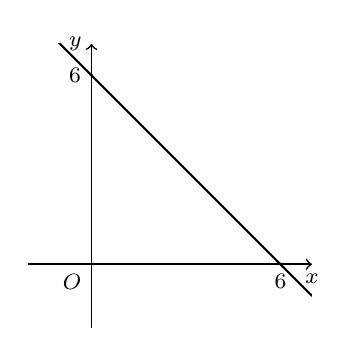
\begin{tikzpicture}[line join=round,line cap=round,line width=.6pt,font=\footnotesize,scale=0.4]
		\def\a{-1} 
		\def\b{6} 
		\draw[->]  (-2,0) -- (7,0) node[below] {$x$};
		\draw[->] (0,-2) -- (0,7)  node[left] {$y$};
		\fill[black] (6,0) node[shift={(-90:6pt)}]{$6$} circle  (1.5pt);
		\fill[black] (0,6) node[shift={(180:6pt)}]{$6$} circle  (1.5pt);
		\draw (0,0) node[below  left]{$O$};
		\clip (-2,-2) rectangle (7,7); 
		 \draw[thick,samples=150,smooth,domain=-2:7] plot (\x,{\a*\x+(\b)});
	\end{tikzpicture}
		} 
	} 
\end{ex}


%%%%%%%%%%%%%%%% TỰ LUẬN %%%%%%%%%%%%%%%%

% nguồn: Ok_TuanLuan_Toan11_Lan1
\begin{bt}%[1D7H2-3]%[ma:3a221723]
	Cho hàm số $y=\dfrac{2x-1}{x-2}$ có đồ thị $\left(C\right)$. Viết phương trình tiếp tuyến của đồ thị $\left(C\right)$, biết tung độ tiếp điểm bằng $3$. 
	 \loigiai{
		Ta có  $y_0=3\Rightarrow\dfrac{2x_0-1}{x_0-2}=3\Rightarrow x_0=5$.
		\begin{eqnarray*}
			&f'\left(5\right) &  =\lim\limits_{x\rightarrow5}\dfrac{f\left(x\right)-f\left(5\right)}{x-5}\\
			& & =\lim\limits_{x\rightarrow5}\dfrac{\dfrac{2x-1}{x-2}-3}{x-5}\\ 
			& & =\lim\limits_{x\rightarrow5}\dfrac{\dfrac{-x+5}{x-2}}{x-5}\\ 
			&  & =\lim\limits_{x\rightarrow5}\dfrac{-1}{x-2}\\
			&  & =-\dfrac{1}{3}.
		\end{eqnarray*}
		Phương  trình tiếp tuyến cần tìm là $y=-\dfrac{1}{3}(x-5)+3\Leftrightarrow y=-\dfrac{1}{3}x+\dfrac{14}{3}$.
	 }
\end{bt}

% nguồn: Ok_TuanLuan_Toan11_Lan1
\begin{bt}%[1D7H2-3]%[ma:0c00f3bb]
	Cho hàm số $y=-x^3+3x^2+9x-1$ có đồ thị là $(C)$. Tìm hệ số góc lớn nhất của tiếp tuyến tại một điểm $M$ trên  đồ thị $(C)$.
	 \loigiai{
		Gọi điểm $M\left(x_0;y_0\right) \in(C)$  là tọa độ tiếp điểm và $y'=-3x^2+6x+9$.\\
		Hệ số góc của tiếp tuyến tại điểm $M$  là $y'\left(x_0\right)=-3x_o^2+6x_o+9$.\\
		Ta thấy, hệ số góc của tiếp tuyến tại điểm $M$ là một hàm số có đồ thị là một parabol, có đỉnh $S\left(-\dfrac{b}{2a};-\dfrac{\Delta}{4a}\right) \Rightarrow S(1;12)$ và hệ số $a=-3<0$ nên hàm số có giá trị lớn nhất bằng $12$  tại $x_o=1$.\\
		 Vậy hệ số góc lớn nhất của tiếp tuyến là $y'(1)=12$.
	} 
\end{bt}

% nguồn: Ok_TuanLuan_Toan11_Lan1
\begin{bt}%[1D7H2-3]%[ma:00785f5f]
	Cho hàm số $y=f(x)=-2x^3+x$ có đồ thị $(C)$. Viết  phương trình tiếp tuyến của đồ thị $(C)$ tại điểm $M(-2; 14)$.
	 \loigiai{
		Ta có $f^{\prime}(x)=\left(-2x^3+x\right)^{\prime}=-6x^2+1$.  \\
		Hệ số góc của tiếp tuyến của $(C)$ tại  điểm $M(-2; 14)$ là $f^{\prime}(-2)=-6\cdot(-2)^2+1=-23$. \\
		Phương trình tiếp  tuyến của $(C)$ tại điểm $M$ là
		 $$
		y-14=-23(x+2) \Leftrightarrow y=-23 x-32. 
		 $$
	 }
\end{bt}

% nguồn: Ok_TuanLuan_Toan11_Lan2
\begin{ex}%[1D7H2-3]%[ma:8b6e25e4]
	Cho hàm số $y=\dfrac{2x-1}{x-2}$ có đồ thị $\left(C\right)$.  Viết phương trình tiếp tuyến của đồ thị $\left(C\right)$, biết tung độ tiếp điểm bằng $3$.
	 \loigiai{
		Ta có $y_0=3\Rightarrow\dfrac{2x_0-1}{x_0-2}=3\Rightarrow  x_0=5$.
		\begin{eqnarray*}
			&f'\left(5\right)  & =\lim\limits_{x\rightarrow5}\dfrac{f\left(x\right)-f\left(5\right)}{x-5}\\
			 & & =\lim\limits_{x\rightarrow5}\dfrac{\dfrac{2x-1}{x-2}-3}{x-5}\\
			& &  =\lim\limits_{x\rightarrow5}\dfrac{\dfrac{-x+5}{x-2}}{x-5}\\
			& &  =\lim\limits_{x\rightarrow5}\dfrac{-1}{x-2}\\
			& & =-\dfrac{1}{3}. 
		\end{eqnarray*}
		Phương trình tiếp tuyến cần tìm là  $y=-\dfrac{1}{3}(x-5)+3\Leftrightarrow y=-\dfrac{1}{3}x+\dfrac{14}{3}$.
	 }
\end{ex}

% nguồn: Ok_TuanLuan_Toan11_Lan2
\begin{ex}%[1D7H2-3]%[ma:2ca9e3a7]
	Cho hàm số $y=-x^3+3x^2+9x-1$ có đồ thị là $(C)$. Tìm hệ số góc lớn nhất của tiếp tuyến tại một điểm $M$ trên đồ thị  $(C)$.
	 \loigiai{
		Gọi điểm $M\left(x_0;y_0\right)  \in(C)$ là tọa độ tiếp điểm và $y'=-3x^2+6x+9$.\\
		Hệ số góc của tiếp tuyến tại điểm $M$ là $y'\left(x_0\right)=-3x_o^2+6x_o+9$.\\ 
		Ta thấy, hệ số góc của tiếp tuyến tại điểm $M$ là một hàm số có đồ thị là một parabol, có đỉnh $S\left(-\dfrac{b}{2a};-\dfrac{\Delta}{4a}\right) \Rightarrow S(1;12)$ và hệ số $a=-3<0$ nên hàm số có giá trị lớn nhất  bằng $12$ tại $x_o=1$.\\
		Vậy hệ số góc lớn nhất của tiếp tuyến là  $y'(1)=12$.
	 }
\end{ex}

% nguồn: Ok_TuanLuan_Toan11_Lan2
\begin{ex}%[1D7H2-3]%[ma:9421b2b0]
	Cho hàm số $y=f(x)=-2x^3+x$ có  đồ thị $(C)$. Viết phương trình tiếp tuyến của đồ thị $(C)$ tại điểm $M(-2; 14)$.
	\loigiai{ 
		Ta  có $f^{\prime}(x)=\left(-2x^3+x\right)^{\prime}=-6x^2+1$. \\
		Hệ số góc của tiếp tuyến của $(C)$ tại điểm $M(-2; 14)$ là $f^{\prime}(-2)=-6\cdot(-2)^2+1=-23$.  \\
		 Phương trình tiếp tuyến của $(C)$ tại điểm $M$ là
		$$ 
		y-14=-23(x+2) \Leftrightarrow y=-23 x-32. 
		$$ 
	} 
\end{ex}

% nguồn: Ok_TuanLuan_Toan11_Lan2
\begin{ex}%[1D7H2-3]%[ma:03be0330]
	Gọi $ M$ là giao điểm của đồ thị hàm số $ y=\dfrac{x+1}{x-2}$ với trục hoành. Viết phương trình tiếp tuyến của đồ thị hàm số trên tại điểm $  M$.
	 \loigiai{
		 Hoành độ điểm $ M$ là nghiệm của phương trình $\dfrac{x+1}{x-2}=0\Leftrightarrow x=-1.$\\
		 Do đó $ M(-1;0)$. Mặt khác, $ y'=-\dfrac{3}{(x-2)^2}$ nên $ y'(-1)=-\dfrac{1}{3}$.\\
	Phương trình tiếp tuyến tại $ M$ là $ y=-\dfrac{1}{3}(x+1)+0\Leftrightarrow 3y+x+1=0$.} 
\end{ex}

% nguồn: Ok_TuanLuan_Toan11_Lan2
\begin{ex}%[1D7H2-3]%[ma:b5931d8c]
	Viết phương trình tiếp tuyến của đồ thị hàm số $ (C)\colon y=x^3-3x+1$ tại giao  điểm của $(C)$ với trục $ Oy$.
	 \loigiai{
		 Ta có $ y'=3x^2-3$.\\
		Giao  điểm $ M$ của đồ thị hàm số $(C)$ với trục $ Oy$ là $x_0=0\Rightarrow y_0=1$.\\
		Hệ  số góc của tiếp tuyến tại $ M\left(0;1\right)$ là $ k=y'(0)=-3$.\\
	 Phương trình tiếp tuyến tại điểm $ M\left(0;1\right)$ là $$ y=k\left(x-x_0\right)+y_0\Leftrightarrow y=-3x+1.$$}
\end{ex}

% nguồn: Ok_TuanLuan_Toan11_Lan2
\begin{ex}%[1D7H2-3]%[ma:4439f25d]
	Cho hàm số $y=x^2+3x+4$ có đồ thị $(C)$. Tính hệ số góc $k$ $(k > 0)$ của tiếp tuyến với đồ thị $(C)$ tại điểm có tung độ bằng $4$. 
	\loigiai{ 
		Ta có hoành độ tiếp điểm của tiếp tuyến là nghiệm của  phương trình $x^2+3x+4=4\Leftrightarrow\hoac{&x=0\\&x=-3.}$\\
		 Ta có $y'=2x+3$.\\
		Với $ x=0$ hệ số góc của tiếp tuyến là $ k=y'(0)=3$.\\ 
	Với $ x=-3$ hệ số góc của tiếp  tuyến là $ k=y'\left(-3\right)=-3$.}
\end{ex}

% nguồn: Ok_TuanLuan_Toan11_Lan2
\begin{ex}%[1D7H2-3]%[ma:fa11e669]
	Cho hàm số $ y=x^4+2x^2$ có đồ thị $(C)$. Viết phương trình tiếp tuyến của  đồ thị $(C)$ tại $ M\left(1;3\right)$.
	 \loigiai{
		Ta có  $y'=4x^3+4x\Rightarrow y'(1)=8$.\\
		 Phương trình tiếp tuyến của đồ thị $(C)$ tại $ M\left(1;3\right)$ là
	$$  y=8\left(x-1\right)+3\Leftrightarrow y=8x-5.$$}
\end{ex}

% nguồn: Ok_TuanLuan_Toan11_Lan2
\begin{ex}%[1D7H2-3]%[ma:5da7dcf6]
	Viết phương trình  tiếp tuyến của đồ thị hàm số $ y=-x^3+2x-1$ tại điểm $ M(1;0)$.
	 \loigiai{
		 Ta có $ y'=-3x^2+2$.\\
		Phương trình tiếp tuyến của đồ thị hàm số $ y=-x^3+2x-1$ tại điểm  $ M(1;0)$ là
		$$ y=y'(1)(x-1)+0=-x+1.$$ 
	 }
\end{ex}

% nguồn: Ok_TuanLuan_Toan11_Lan2
\begin{ex}%[1D7H2-3]%[ma:aeb2666f]
	Viết phương trình tiếp tuyến của đồ thị hàm số $ y=x^3$ tại điểm  $\left(-1;-1\right)$.
	 \loigiai{
		Ta có  $ y'=3x^2\Rightarrow y'\left(-1\right)=3$.\\
	Phương trình tiếp tuyến  là $ y=3\left(x+1\right)-1=3x+2$.}
\end{ex}

% nguồn: Ok_TuanLuan_Toan11_Lan2
\begin{ex}%[1D7H2-3]%[ma:2c5bc77a]
	 Viết phương trình tiếp của đường cong $ y=x^3$ tại điểm $\left(-2;-8\right)$.
	\loigiai{ 
		Ta  có $ y'=3x^2$.\\
		Khi đó hệ số góc của tiếp tuyến tại điểm $\left(-2;-8\right)$ là  $ y'\left(-2\right)=12$.\\
	Phương trình tiếp tuyến cần tìm là $  y=12\left(x+2\right)-8\Leftrightarrow y=12x+16$.}
\end{ex}

% nguồn: Ok_TuanLuan_Toan11_Lan2
\begin{ex}%[1D7H2-3]%[ma:96225d0e]
	Cho hàm số $ y=x^3-3x+1$. Viết phương trình tiếp tuyến với đồ thị hàm số  tại giao điểm của đồ thị hàm số với trục tung.
	 \loigiai{
		 Ta có $ y'=3x^2-3$.\\
		Đồ thị hàm số cắt  $ Oy$ tại điểm $ A\left(x_0;y_0\right)\Rightarrow x_0 =0\Rightarrow y_0=1$.\\
		Gọi tiếp tuyến $d$ tiếp  xúc đồ thị hàm số tại điểm $ A\left(0;1\right)$.\\
		 Suy ra hệ số góc $ k=y'\left(x_0\right)=y'(0)=-3$.\\
	Vậy  phương trình tiếp tuyến $ d\colon y=-3\left(x-0\right)+1\Leftrightarrow y=-3x+1$.}
\end{ex}

% nguồn: Ok_TuanLuan_Toan11_Lan2
\begin{ex}%[1D7H2-3]%[ma:1c2afd65]
	Viết phương trình tiếp tuyến của đồ thị hàm số  $y=4x^3-6x^2+1$ tại điểm có hoành độ $x=1$.
	\loigiai{ 
		Ta  có $y'=12x^2-12x\Rightarrow y'(1)=0$.\\
		Ta  có $x_0=1\Rightarrow y_{0}=-1$.\\
		Phương trình tiếp  tuyến của đồ thị hàm số $y=4x^3-6x^2+1$ tại điểm có hoành độ $x=1$ là
	 $y=-1$.}
\end{ex}

% nguồn: Ok_TuanLuan_Toan11_Lan2
\begin{ex}%[1D7H2-3]%[ma:ee31dc90]
	Cho hàm số $  y=\dfrac{x+1}{x-1}$ có đồ thị $(C)$. Viết phương trình tiếp tuyến của $(C)$ tại giao điểm của $(C)$ với trục tung.
	 \loigiai{
		Giao điểm của đồ thị $(C)$ và trục tung  là $ M\left(0;-1\right)$.\\
		 Ta có $ y'=\dfrac{-2}{\left(x-1\right)^2}$.\\
		Phương trình tiếp tuyến của $(C)$ tại $ M\left(0;-1\right)$  là
	 $$ y =y'(0)\left(x-0\right)-1=-2x-1.$$}
\end{ex}

% nguồn: Ok_TuanLuan_Toan11_Lan1
\begin{bt}%[1D7V2-3]%[ma:9c96cdc2]
	Cho hàm số $y=\dfrac{9}{x}$ có đồ thị là $(C)$. Biết tiếp  tuyến của đồ thị $(C)$ tại điểm $M(3;3)$ tạo với hai trục toạ độ một tam giác. Diện tích tam giác đó bằng bao nhiêu?
	 \loigiai{
		Ta có $y'=\dfrac{-9}{x^2}$.\\ 
		Hệ số góc của tiếp  tuyến tại điểm $M$ là $y'(3)=\dfrac{-9}{3^2}=-1$.\\
		Phương trình tiếp tuyến $(\Delta)$ với $(C)$ tại tiếp  điểm $M$ là
		\[y-3=-1(x-3)\Leftrightarrow  y=-x+6.
		 \]
		Ta có $(\Delta) \cap Ox = A(6;0)$ và $(\Delta) \cap Oy =  B(0;6)$.\\
		 Tam giác $OAB$ vuông tại $O$ nên có diện tích là
		\[S_{\triangle OAB}=\dfrac{1}{2} OA\cdot OB=\dfrac{1}{2}  \cdot 6\cdot 6=18.
		 \]
	} 
\end{bt}

% nguồn: Ok_TuanLuan_Toan11_Lan2
\begin{ex}%[1D7V2-3]%[ma:008b20e6]
	Cho hàm số $y=\dfrac{9}{x}$ có đồ thị là $(C)$. Biết tiếp tuyến của  đồ thị $(C)$ tại điểm $M(3;3)$ tạo với hai trục toạ độ một tam giác. Diện tích tam giác đó bằng bao nhiêu?
	 \loigiai{
		Ta  có $y'=\dfrac{-9}{x^2}$.\\
		Hệ số góc  của tiếp tuyến tại điểm $M$ là $y'(3)=\dfrac{-9}{3^2}=-1$.\\
		Phương trình tiếp tuyến $(\Delta)$ với $(C)$  tại tiếp điểm $M$ là
		\[y-3=-1(x-3)\Leftrightarrow  y=-x+6.
		\] 
		Ta có $(\Delta) \cap Ox = A(6;0)$ và  $(\Delta) \cap Oy = B(0;6)$.\\
		Tam giác $OAB$ vuông  tại $O$ nên có diện tích là
		\[S_{\triangle OAB}=\dfrac{1}{2} OA\cdot OB=\dfrac{1}{2}  \cdot 6\cdot 6=18.
		\] 
	 }
\end{ex}

% nguồn: Ok_TuanLuan_Toan11_Lan2
\begin{ex}%[1D7V2-3]%[ma:fd05c2d7]
	Cho hàm số $ y=f(x)$ có đạo hàm liên tục trên $ \mathbb{R} $, thỏa mãn $ 2f\left(3x-3\right)+f\left(6-3x\right)=3x^2-5x$. Viết phương trình tiếp tuyến của đồ thị hàm số $ y=f(x)$ tại điểm có hoành độ bằng $ 3  $.
	 \loigiai{
		 Ta có $ 2f\left(3x-3\right)+f\left(6-3x\right)=3x^2-5x$. \hfill $(1)$\\
		Phương trình tiếp tuyến của đồ thị hàm số $ y=f(x)$ tại điểm có hoành độ bằng  $ 3 $ có dạng
		$$  y=f'(3)\left(x-3\right)+f(3).$$
		Thay $ x=1$ vào $ (1) $  ta được $ 2f(0)+f(3)=-2$. \hfill $(2)$\\
		Thay  $ x=2$ vào $ (1) $ ta được $ 2f(3)+f(0)=2$. \hfill $(3)$\\
		Từ $ (2) $ và $ (3) $ suy  ra $ f(3)=2$.\\
		Lấy đạo  hàm hai vế của $ (1) $ ta được $ 6f'\left(3x-3\right)-3f'\left(6-3x\right)=6x-5$. \hfill $(4)$\\
		Thay $ x=1$ vào $ (4) $ ta  được $ 6f'(0)-3f'(3)=- 5$. \hfill $(5)$\\
		Thay $ x=2$ vào  $ (4) $ ta được $ 6f'(3)-3f'(0)=7$. \hfill $(6)$\\
		Từ $ (5) $ và $ (6) $ suy  ra $ f'(3)=1$.\\
		Vậy phương trình tiếp tuyến  của đồ thị hàm số $ y=f(x)$ tại điểm có hoành độ bằng $ 3 $ là
	$$  y=1\left(x-3\right)+2=x-1.$$}
\end{ex}

% nguồn: Ok_TuanLuan_Toan11_Lan2
\begin{ex}%[1D7V2-3]%[ma:c26e4998]
	 Cho hàm số $ y=f(x)$ có đạo hàm liên tục trên $ \mathbb{R} $, thỏa mãn $ 2f(5-x)+xf(x)=2x$. Viết phương trình tiếp tuyến của đồ thị hàm số $ y=f(x)$ tại điểm có hoành độ bằng $ 5$.
	\loigiai{ 
		Thay $ x=0$ vào $ 2f(5-x)+xf(x)=2x$ ta được  $ 2f(5)=0\Rightarrow f(5)=0$.\\
		Thay $  x=5$ vào $ 2f(5-x)+xf(x)=2x$ ta được $ 2f(0)+5f(5)=10\Rightarrow f(0)=5$.
		$$ 2f(5-x)+xf(x)=2x\Rightarrow-2f'(5-x)+f(x)+xf'(x)=2.  \qquad (*)$$
		Thay $ x=0$ vào $ (*)$ ta có $-2f'(5)+f(0)=2\Rightarrow f'(5)=\dfrac{3}{2}$.\\ 
	Vậy phương trình tiếp tuyến của đồ thị  hàm số $ y=f(x)$ tại điểm có hoành độ là $ 5$ là $$ y=f'(5)(x-5)+f(5)=\dfrac{3}{2}(x-5)+0=\dfrac{3}{2}x-\dfrac{15}{2}.$$}
\end{ex}
